\documentclass[]{article}
 \usepackage{hyperref}
 \hypersetup{
 	colorlinks=true,
 	linkcolor=blue,
 	filecolor=blue,      
 	urlcolor=blue,
 	citecolor=blue
 }
 \usepackage{natbib}
 \usepackage{graphicx}
 \usepackage{caption}
 \usepackage{subcaption}
 
%opening
\title{Perceived Income Risks}
\author{Tao Wang}

\begin{document}

\maketitle

\begin{abstract}
This is a research proposal. Econometricians have long estimated the parameters of an income process relying upon moment restrictions imposed on \textit{only} realized income series.  Density forecasts of individual income growth provide directly measured perceived income risks, and it helps econometricians uncover the income process and estimate the size of the permanent/transitory risks better. In the same time, comparing the perception and econometrical estimation is a straightforward way to characterizes how the expectation formation of agents deviates from the benchmark of rational expectation. After establishing patterns of the hetergeneity in perceived income risks, I will also look into its impacts on economic decisions. As a final step, the discovered patterns of perceived income risks can be incoporated into an otherwise standrad life-cycle models with heterogeneous agents to examine their macroeconomic implications. 
 
\end{abstract}

\section{Introduction}


Even if two agents share the same mean expectated income, the difference in magnitude of conditional variance of the income, i.e. income risks, have a non-trivial impacts on the decisions of the agents. For instance, precautionary saving arises when agents are faced with a mean-preserving spread of income compared to its certainty counterpart in a non-quadradic utility function. 

Expectation data, especially the directly estimated perceived income risks from surveys provide additional moments for identification. It allows for differentiating insurence from information (\citet{kaufmann_disentangling_2009}, \citet{meghir_chapter_2011}). For instance, the well-known empirical finding of excessive sensitivity may be either due to the limited insurance, or due to the unexpected nature of the shocks. What economists typically do is to intereprete the empirical evidence via the first by making rationality assumptions about the second. 

This paper is related to three lines of literature. First, the literature that studies the expectations of economic agents. Most of this literature focues on the firs moment of the expectations, i.e. mean value. The availability of income risks allows for studying the second moments of income, i.e. variances, namely income risks. The most relevant work includes \citet{rozsypal2017overpersistence}, where the authors compare expected income growth with realized income growth in the survey data, finding evidence for what is called ``overpersistence bias'' by agents. 

Second, the literature on expectation formation in general. This paper focuses on micro variable instead of macro. Relative to macro variables, idiosyncratic variables are more generally more relevant to individual decisions. 

Third, the literature that develped under the standard onconsumption/saving models with uninsured income risks. 


\section{Stylized Facts}

Figure \ref{SCEPopTS} plots the median value of mean, variance and inter-range quantile of expected income growth from SCE.  

	\begin{figure}[ht]
	
		\centering
		\caption{Expected Income Growth }
		\label{SCEPopTS}
		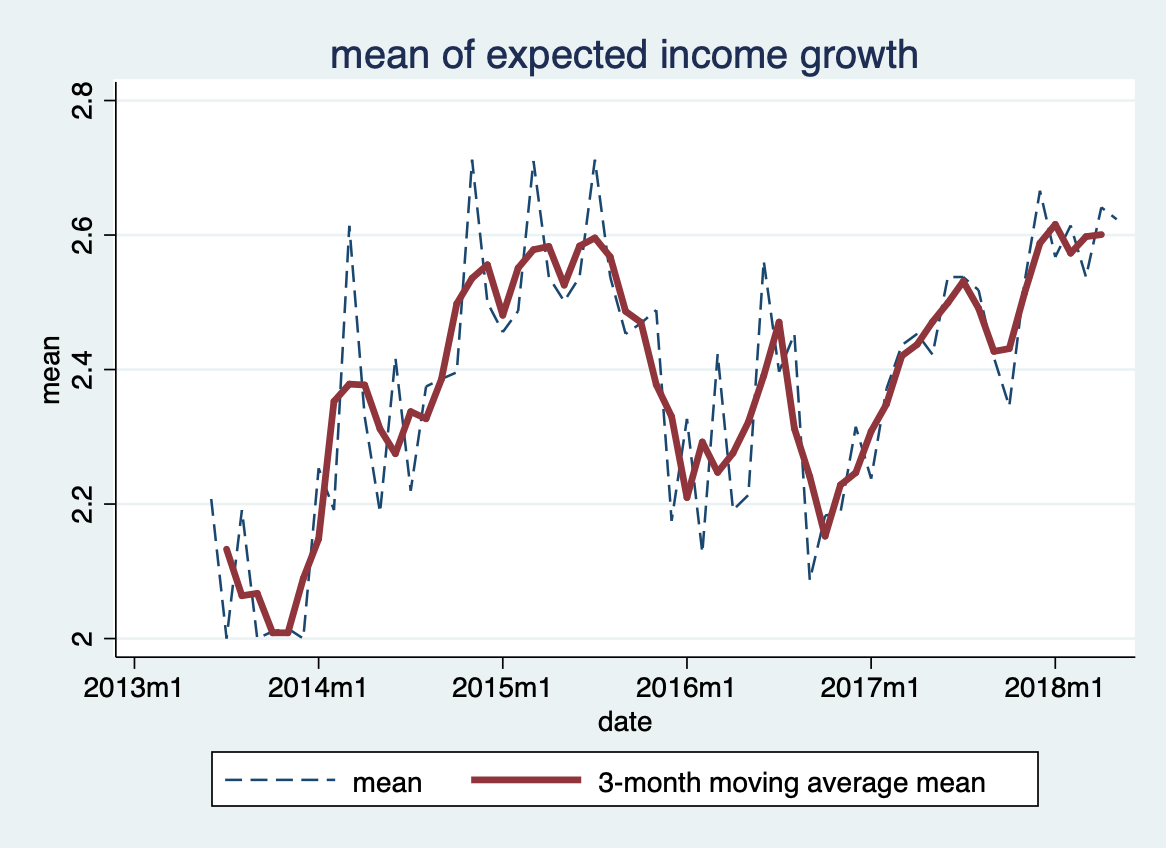
\includegraphics[width=0.3\textwidth]{figures/median_mean.png}
		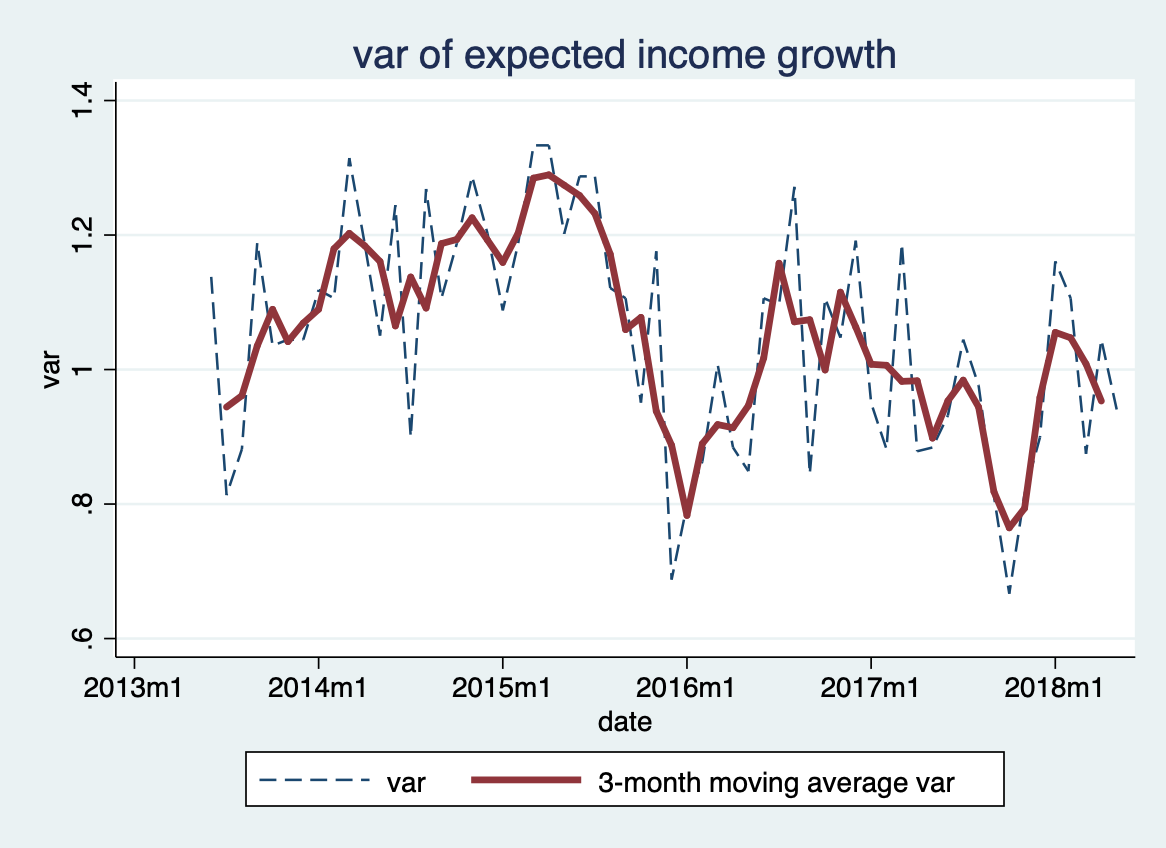
\includegraphics[width=0.3\textwidth]{figures/median_var.png}
		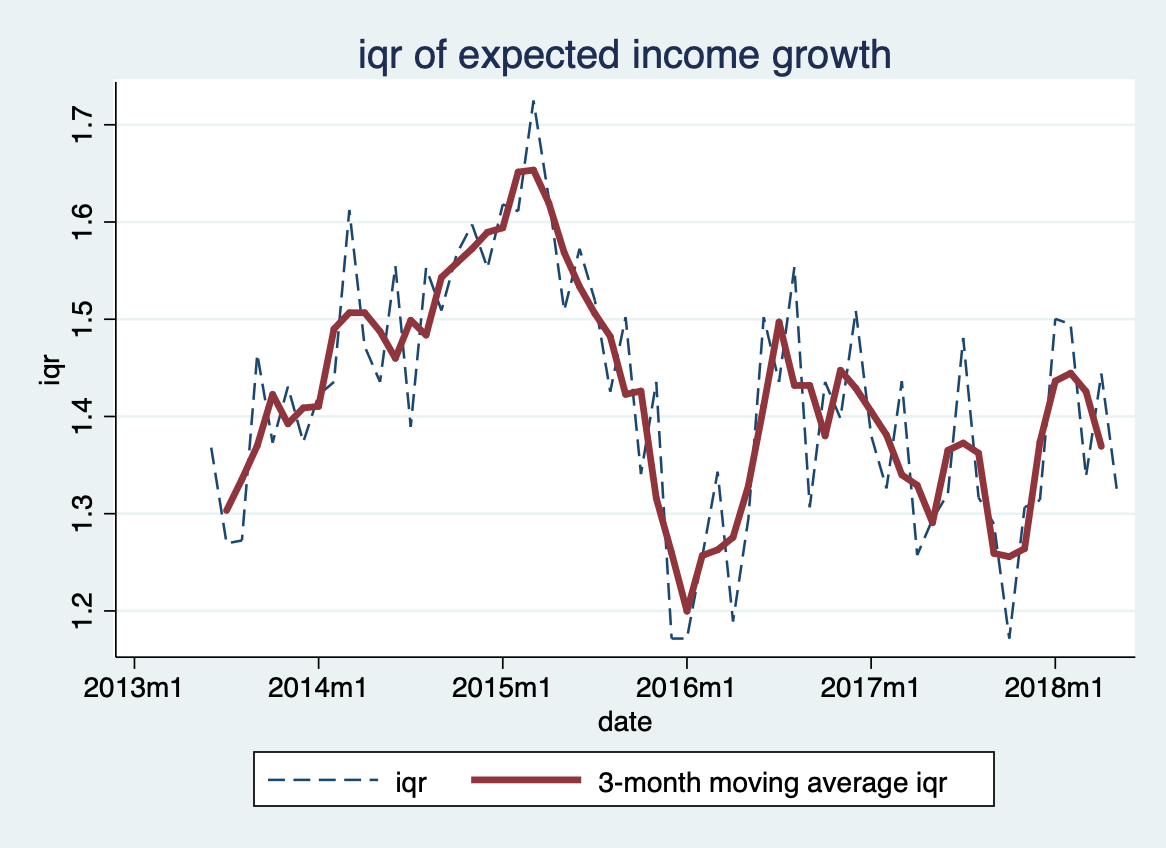
\includegraphics[width=0.3\textwidth]{figures/median_iqr.png}
	\begin{flushleft}
		{\footnotesize Note: the dashed line is monthly, and the solid line is 3-month moving average. }
	\end{flushleft}

\end{figure}


Figure \ref{SCEPopHist} plots the distribution of perceived income risks across all participants of the survey. 


\begin{figure}[ht]
	
	\centering
	\caption{Distribution of Perceived Income Growth and Income Risks}
	\label{SCEPopHist}
	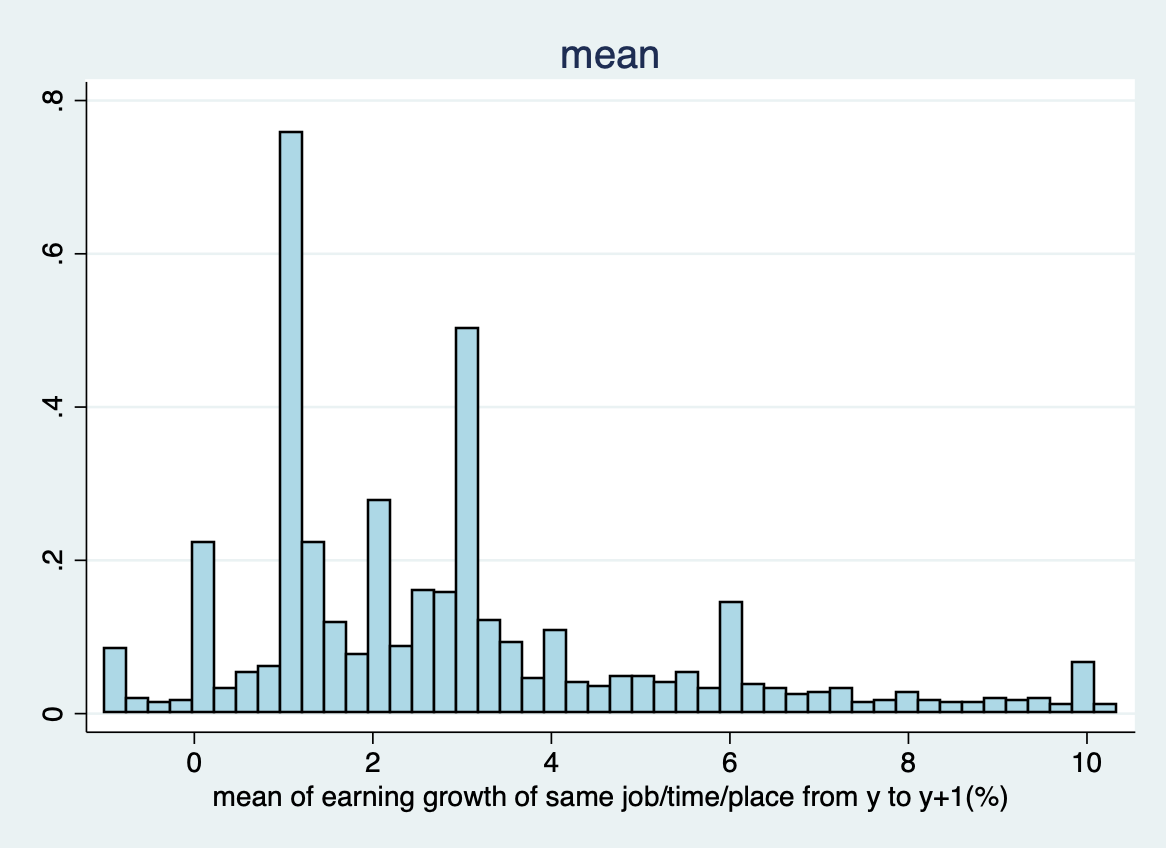
\includegraphics[width=0.3\textwidth]{figures/hist_mean.png}
	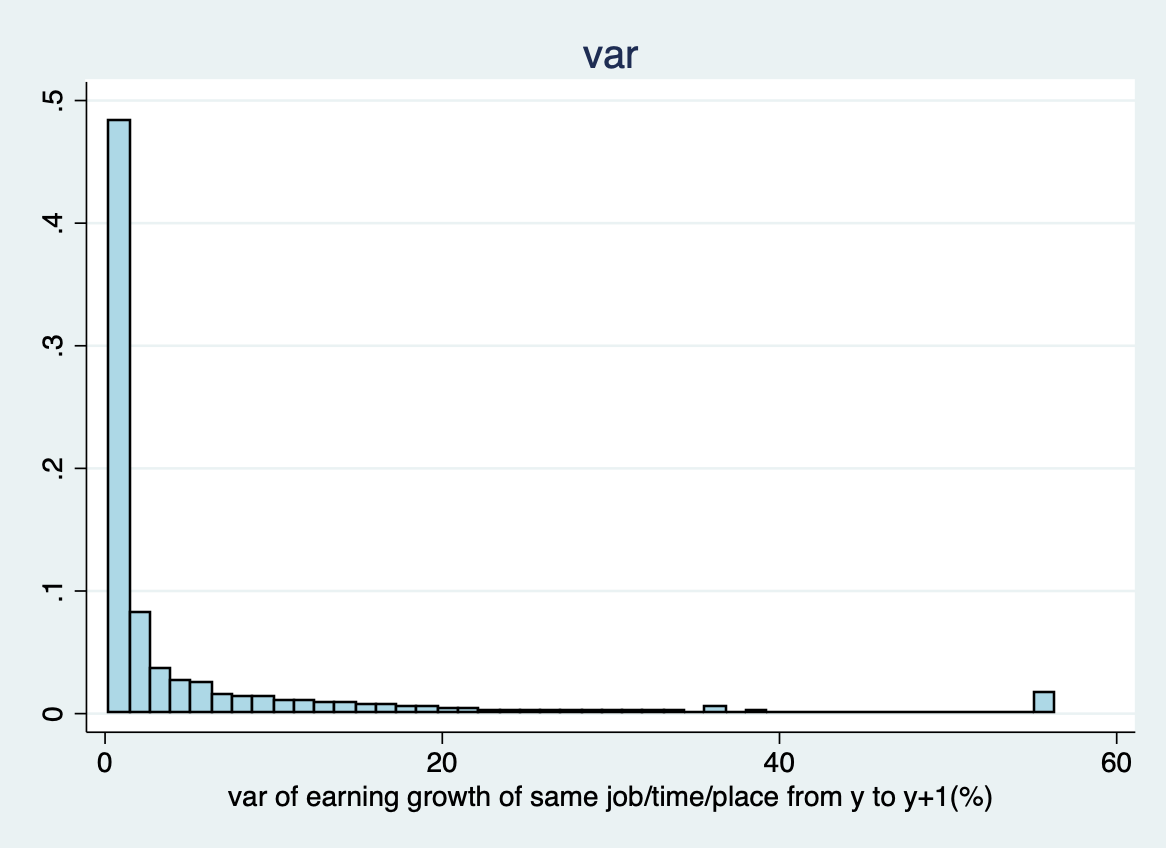
\includegraphics[width=0.3\textwidth]{figures/hist_var.png}
	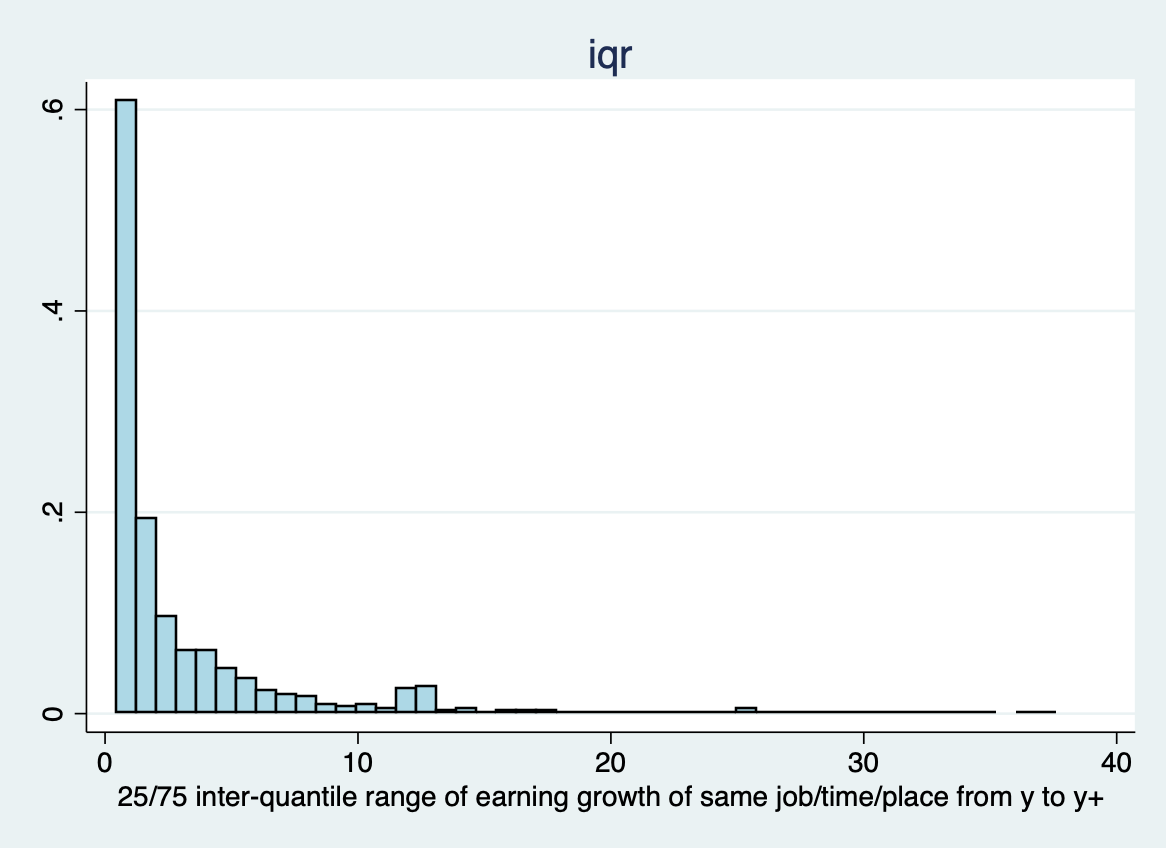
\includegraphics[width=0.3\textwidth]{figures/hist_iqr.png}
	\begin{flushleft}
		{\footnotesize Note: }
	\end{flushleft}
	
\end{figure}

Figure \ref{SCEPopHist_byGroup} plots the distribution of perceived income risks by different groups. 

\begin{figure}[ht]
	
	\centering
	\caption{Distribution of Perceived Income Risks by Demographical Groups}
	\label{SCEPopHist_byGroup}
	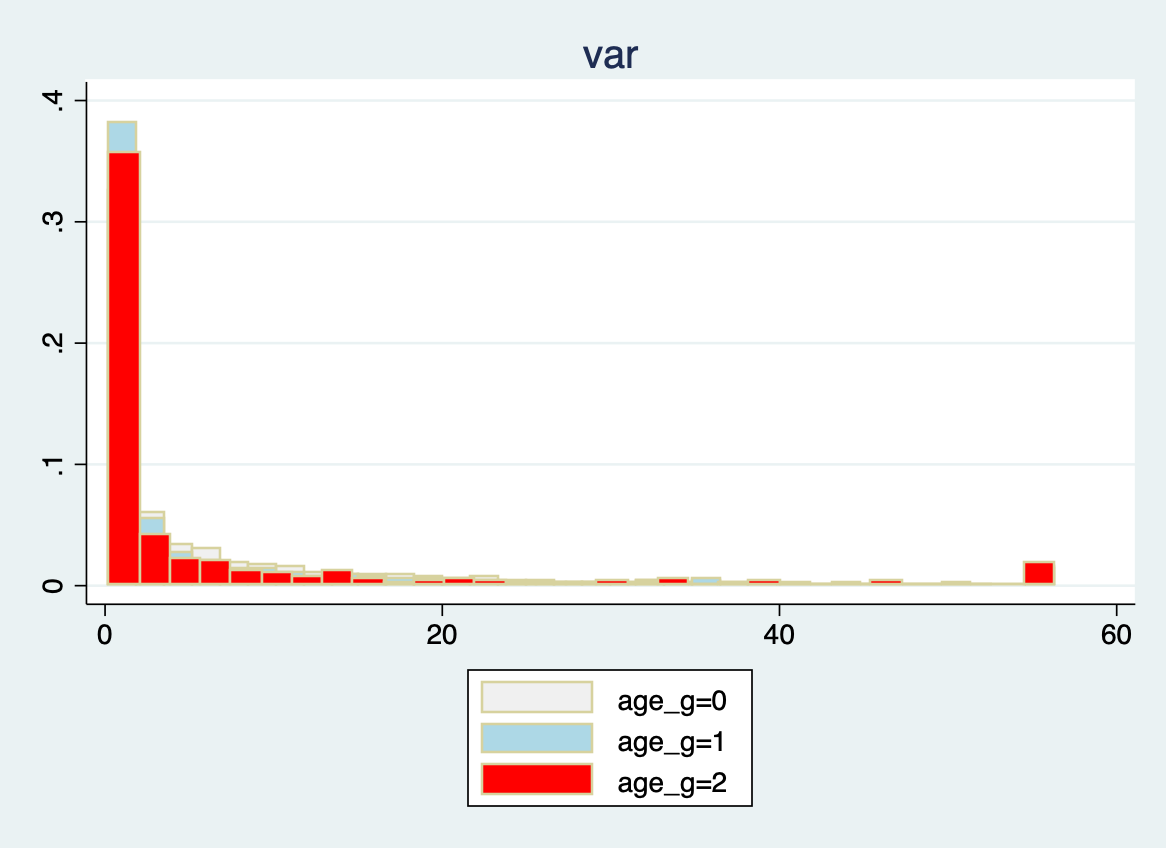
\includegraphics[width=0.3\textwidth]{figures/hist_var_age_g.png} \\
	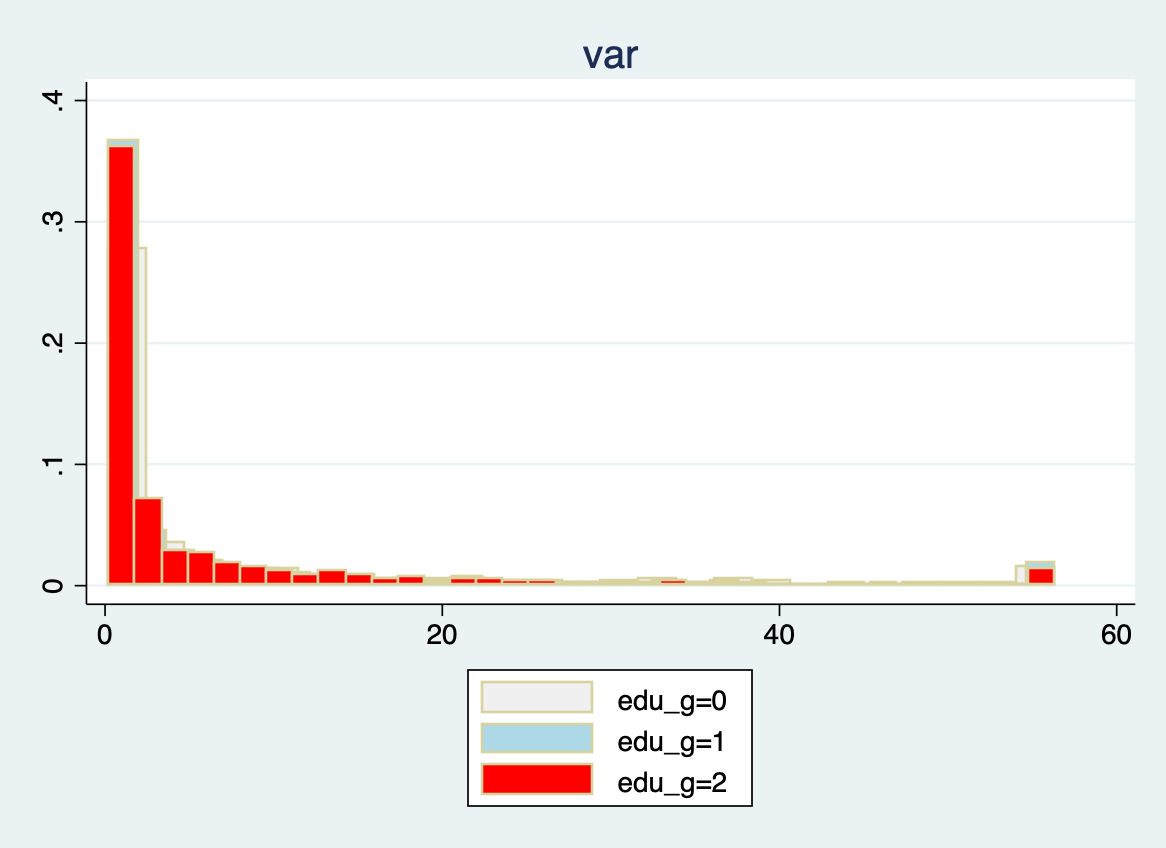
\includegraphics[width=0.3\textwidth]{figures/hist_var_edu_g.png} \\
	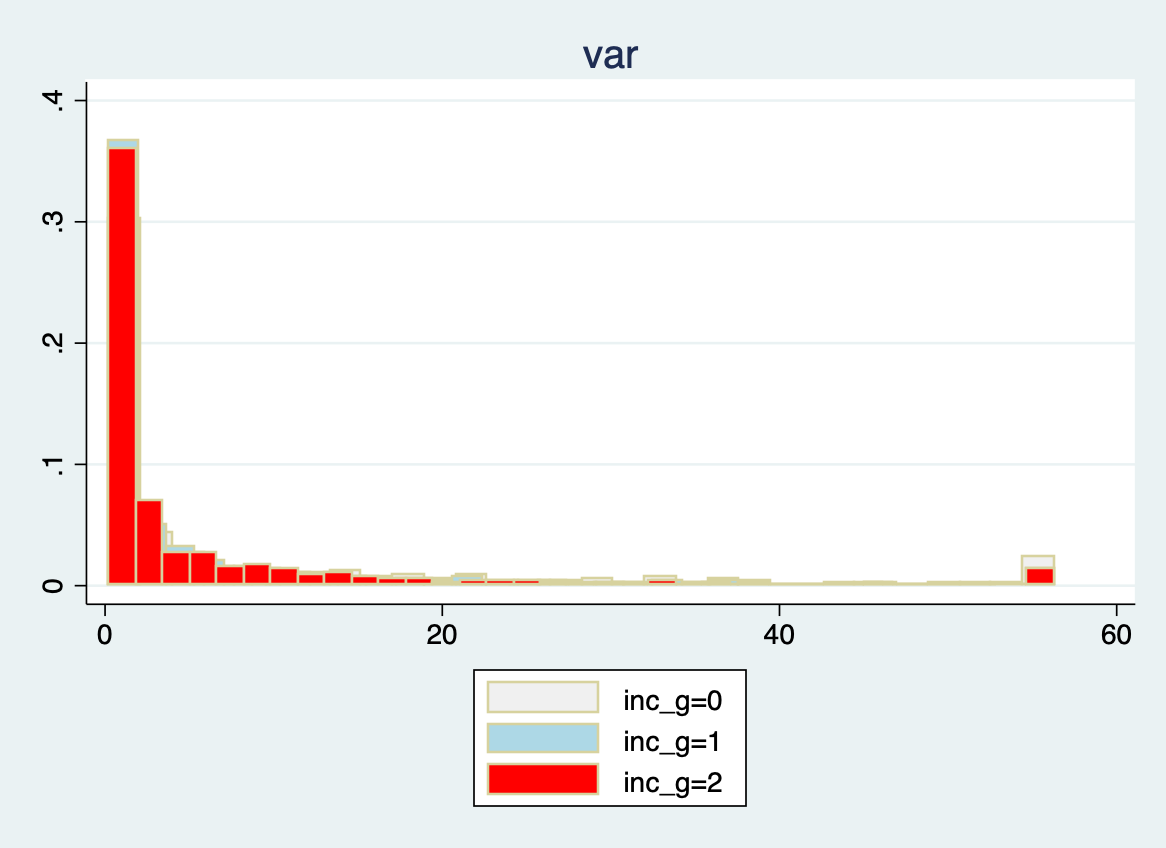
\includegraphics[width=0.3\textwidth]{figures/hist_var_inc_g.png}
	\begin{flushleft}
		{\footnotesize Note: }
	\end{flushleft}
	
\end{figure}

\bibliographystyle{apalike}
\bibliography{PerceivedIncomeRisks}

\end{document}
